\documentclass[conference]{IEEEtran}

\usepackage{cite}
\usepackage[utf8]{inputenc}
\usepackage[absolute]{textpos}
\usepackage{graphicx}
\usepackage{hyperref}

% Remove boxes from links
\usepackage{xcolor}
\hypersetup{
    colorlinks,
    linkcolor={red!50!black},
    citecolor={blue!50!black},
    urlcolor={blue!80!black}
}

\ifCLASSINFOpdf
  
\else
 
\fi


% If necessary, add hyphenations here
\hyphenation{}

\begin{document}
\vspace{50mm}

% Report header (Title, authors, ...)
\title{soHappy}

\author{
  \IEEEauthorblockN{
    \textbf{Marcel Arndt}
  }
  \IEEEauthorblockA{
    Hochschule Augsburg \\
    Augsburg, Germany \\
  } \and
  \IEEEauthorblockN{
    \textbf{Lukas Diehm}
  }
  \IEEEauthorblockA{
    Hochschule Augsburg \\
    Augsburg, Germany \\
  } \and
  \IEEEauthorblockN{
    \textbf{Anna Gsell}
  }
  \IEEEauthorblockA{
    Hochschule Augsburg \\
    Augsburg, Germany \\
  } \and
  \IEEEauthorblockN{
    \textbf{Kok Yew Lim}
  }
  \IEEEauthorblockA{
    Hochschule Augsburg \\
    Augsburg, Germany \\
  } \and
  \IEEEauthorblockN{
    \textbf{Fabian Siegel}
  }
  \IEEEauthorblockA{
    Hochschule Augsburg \\
    Augsburg, Germany \\
  }
}

\maketitle

% University logo
\begin{textblock*}{188mm}(55mm,11mm)

\includegraphics[width=0.55\textwidth]{figures/informatik_Logo.jpg}
\end{textblock*}

% Abstract
\begin{abstract}

Lorem ipsum dolor sit amet, consetetur sadipscing elitr, sed diam nonumy eirmod tempor invidunt ut labore et dolore magna aliquyam erat, sed diam voluptua. At vero eos et accusam et justo duo dolores et ea rebum. Stet clita kasd gubergren, no sea takimata sanctus est Lorem ipsum dolor sit amet. Lorem ipsum dolor sit amet, consetetur sadipscing elitr, sed diam nonumy eirmod tempor invidunt ut labore et dolore magna aliquyam erat, sed diam voluptua. At vero eos et accusam et justo duo dolores et ea rebum. Stet clita kasd gubergren, no sea takimata sanctus est Lorem ipsum dolor sit amet.

\end{abstract}


\IEEEpeerreviewmaketitle

% Main chapters
\section{Introduction} \label{sec:introduction}
With technology steadily improving over the years, people are becoming more interconnected than ever and entertainment in form of applications are plentiful. Despite this, depression continues to rise among the general population. According to the World Health Organization, over 322 million cases of depressive disorder were recorded in 2017, representing a rise of around 18.4\% over the past ten years \cite{who_depression}. Not only does depression negatively impact wellbeing, it may also lead to complications such as increased fatigue, decreased motivation or even suicide. As a result, researchers have used computing technologies known as \textit{Affective Computing} that seek to identify human emotions in order to combat mental disorders \cite{ieee_affective}.

In \cite{sohappy}, Moore, Galway and Donnelly propose a smartphone application to be used in a future study. It is designed to encourage smiling, which has been shown to positively affect happiness and thus serves as an effective means to counteract depression. The research objective of this report is to design and implement the approach described by Moore, Galway and Donnelly as an Android application. In order to render the application suitable for different kinds of studies, the application's components are designed to be as interchangeable as possible, allowing individual adjustments to be made with ease.

The report starts with an overview of appropriate approaches to implement the application in Section \ref{sec:background}. In Section \ref{sec:methodology}, the design choices and architecture of the app are described in detail, followed by a description of the implementation details in Section \ref{sec:implementation}. After presenting the development outcome in Section \ref{sec:results} and a discussion about alternative approaches in Section \ref{sec:discussion}, Section {sec:conclusion} concludes the report with ideas for further work on the app.


\section{Background} \label{sec:background}
% identifying existing approaches within the research literature; this may potentially include mobile-based and non-mobile approaches if necessary
Since Viola and Jones proposed ``Rapid Object Detection using a Boosted Cascade of Simple Features'' in 2001, their concept is the basis of most face detection approaches.
It's an extremely fast and solid machine learning approach for object detection in videos and pictures, e. g. faces.

In detail, the concept is distinguished by three key components.
The first is the “Integral Image”, a new image representation which allows the detector to compute features very fast.
Secondly an AdaBoost based learning algorithm selects a small number of promising visual features and constructs very efficient classifiers.
The last component is a method which combines increasingly more complex classifiers in a “cascade” where most of the computation time is spent on critical object-like parts of the given image by discarding non-promising regions early in the analysis process \cite{viola_jones}.

For that reason the approach is highly appropriate to fulfill the face detection task of the soHappy application.
The open source computer vision and machine learning software library OpenCV provides a cascade classifier class for object detection, which uses the concept of Viola and Jones \cite{opencv_cascade_classifier}.


\section{Methodology} \label{sec:methodology}
% detailing the approaches that were used in your experiments; this may also include implementation details in relation to the mobile architecture used
According to \cite{sample_ref}, lorem ipsum dolor sit amet, consetetur sadipscing elitr, sed diam nonumy eirmod tempor invidunt ut labore et dolore magna aliquyam erat, sed diam voluptua. At vero eos et accusam et justo duo dolores et ea rebum. Stet clita kasd gubergren, no sea takimata sanctus est Lorem ipsum dolor sit amet. Lorem ipsum dolor sit amet, consetetur sadipscing elitr, sed diam nonumy eirmod tempor invidunt ut labore et dolore magna aliquyam erat, sed diam voluptua. At vero eos et accusam et justo duo dolores et ea rebum. Stet clita kasd gubergren, no sea takimata sanctus est Lorem ipsum dolor sit amet. Lorem ipsum dolor sit amet, consetetur sadipscing elitr, sed diam nonumy eirmod tempor invidunt ut labore et dolore magna aliquyam erat, sed diam voluptua. At vero eos et accusam et justo duo dolores et ea rebum. Stet clita kasd gubergren, no sea takimata sanctus est Lorem ipsum dolor sit amet.

\subsection{User Journey} \label{sec:user_journey}
Upon launching the soHappy app, the user will be presented with a home screen, where they can either start the app or navigate to miscellaneous screens via an options menu in which the user may change settings, for example.
When the user starts the app, they will be asked to move their face into the camera frame.

Once a face has been detected, a countdown of three seconds is started, allowing the user to relax and take a couple of breaths. After the countdown has expired, the user will be asked to smile for a set number of seconds. Visual feedback is provided to the user once a smile has been detected.
By virtue of the user seeing their own face during this process, genuine smiling may become difficult, especially if the user has problems with feelings of self-consciousness. In order to assist the user in smiling, a stimulus is shown on the screen, telling the user to recall memories they are fond of. Furthermore, a color filter is applied to the camera, rendering objects harder to recognize.
Should the user fail to smile for at least ten seconds after their face has been detected, the process will be canceled. From this point, the user may opt to try again or continue on to the next part.

Following this process, a set of six questions querying current circumstances are posed to the user, which they are asked to answer. Once all questions have been answered, the user will be thanked for their participation and presented with a percentage indicating how likely they are genuinely happy.

\subsection{Architecture}
Lorem ipsum dolor sit amet, consetetur sadipscing elitr, sed diam nonumy eirmod tempor invidunt ut labore et dolore magna aliquyam erat, sed diam voluptua. At vero eos et accusam et justo duo dolores et ea rebum.

\subsection{State Machine}
Lorem ipsum dolor sit amet, consetetur sadipscing elitr, sed diam nonumy eirmod tempor invidunt ut labore et dolore magna aliquyam erat, sed diam voluptua. At vero eos et accusam et justo duo dolores et ea rebum.

\subsection{User Interface} \label{sec:user_interface}
Like most smartphone applications, the soHappy app consists of multiple screens that the user can navigate through, each of them serving a different purpose. Such screens can be implemented in Android using the \texttt{Activity} and \texttt{Fragment} classes. An \texttt{Activity} object acts as an entry point to an Android app and provides a window for User Interface components to be created in \cite{intro_to_activities}. \texttt{Fragment} objects largely fulfill the same task, but are distinct from \texttt{Activity} objects in that they cannot persist on their own and must be hosted within an \texttt{Activity} object \cite{intro_to_fragments}. Since the soHappy app can only be started manually, a single \texttt{Activity} object for its sole entry point is sufficient. Each screen within the app is implemented with a \texttt{Fragment} object, which is hosted inside the single \texttt{Activity}. An example of how \texttt{Fragment} objects are implemented is shown in figure \ref{fig:user_interface}.

\begin{figure}
  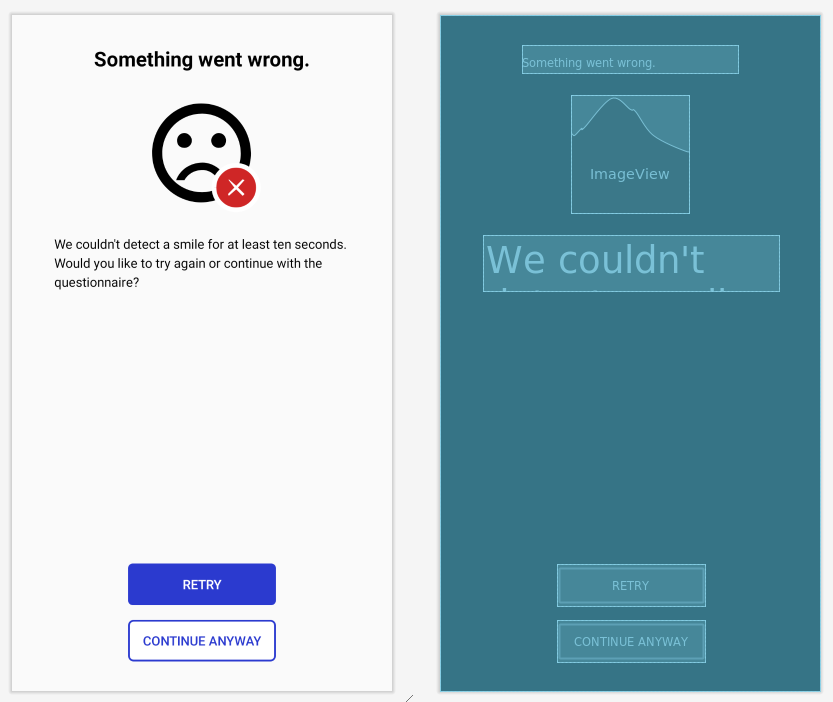
\includegraphics[width=\linewidth]{figures/user_interface.png}
  \caption{Example of a UI fragment designed in Android Studio's Layout Editor. A rendered screen is shown on the left, while its blueprint is depicted on the right.}
  \label{fig:user_interface}
\end{figure}

In terms of design, Android apps are generally expected to conform to Material Design, a set of guidelines defined by Google to help ensure both visual and practical consistency. As such, the user interface of the soHappy app is designed with Material Design in mind \cite{material_design}, incorporating principles such as animation or design based on the real world.

\subsection{Model Training}

As stated in the background section, soHappy uses a deep learning model to 
provide information about a person smiling by utilizing TFLite.

However, for TFLite to detect smiling, the model must be trained first. This
model is not trained on the device, but will be trained in before and shipped
with the android app.

The soHappy smile detection model is on based a convolutional neural network 
(CNN). CNNs are useful for image analysis purposes. A CNN utilizes multiple
convolutional layers as well as pooling layers. A convolutional layer works by
applying multiple different filters onto the input of the layer. A 
convolutional layer also looks at regions of the applied filter layers instead 
of individual pixels. This process is called convolution.
Pooling describes the process of discarding unused information.
Refer to \cite{8308186} for a more in-depth explanation on how CNNs work.

For the soHappy smile detection model, eight convolutional layers are used. 
Every two consecutive convolutional layers are followed by a pooling layer, 
repeated four times. In the end, a the result is flattened. This model
architecture is based on the work of Madnani \cite{MayurMadnani2018}.

In order to train the model, the dataset of \cite{Arigbabu2015} was utilized.
\section{Implementation} \label{sec:implementation}

The app is built using Kotlin. Kotlin is ``[...] an open-source statically 
typed programming language that targets the JVM, Android, JavaScript and 
Native.'' \cite{kotlin2020}
Google officially supports Kotlin for Android apps since 2017
\cite{googleio2017} and recommends using Kotlin since 2019
\cite{androidkotlin2019}.

Thanks to the similarity with languages like Java and TypeScript, adapting
Kotlin as programming language was relatively easy for the project team.

Various language features of Kotlin helped in development, too. Instead of
implementing the singleton pattern, Kotlin allows to create an single object
per runtime by using the \texttt{object}-Keyword.

Some design choices of the app were slowed down by Kotlin's language features.
As all Kotlin classes inherit from \texttt{Any}, using features of Java's 
\texttt{Object}-class are not natively available. This made using the methods
\texttt{.wait()} and \texttt{.notify()}, which are used for synchronisation,
more difficult.

``Android Studio'', known as the official integrated development environment 
(IDE) for Android development, allowed faster development thanks to useful
features like auto-completion. 

An Android app is built into an `apk'-file. In order to reduce application
size, soHappy differentiates between CPU architectures, and will
build an apk for each architecture. As a minimum SDK version, version 23
is selected. This means that the app works on Android 6 and above.

In order to improve the code quality, a linting software called ``detekt'',
``[...] a static code analysis tool [...]''\cite{detekt2020} was used.

Various libraries were used to help implement the application. Using
the included build tool ``Gradle'' \cite{gradle} allowed easy management of 
dependencies. The following libraries are worth mentioning: CameraX 
\cite{camerax} is Android's newest library allowing access to the camera and 
providing an easy way to analyse captured images. ``GPUImage'' \cite{gpuimage}
allowed to apply filters onto the preview image. A library called ``Nitrite''
\cite{nitrite} allows to implement an NoSQL-Database storing our measurement 
locally.

For image analysis, we used the following libraries: Cascade based face
detection use the official `OpenCV4Android'-Library \cite{opencv4android}.
while machine learning based approaches utilise the official TFLite library.
\cite{tensorflow}

In order to train the CNN, which is explained in \ref{sec:methodology}, a
Python 3 script running in an Jupyter notebook was utilised. 
The Python TensorFlow library was used in combination with `Keras',
which allows creating an model architecture easily. In order to prepare the
training, test and validation data, the libraries `pandas', `pillow', 
`mathplotlib' and `numpy' were used.

\section{Results} \label{sec:results}
% some sort of visualisation of the results from research and/or results from the implementation of the mobile app
Lorem ipsum dolor sit amet.


\section{Discussion} \label{sec:discussion}
% analysis and consideration of the results presented in the Results section
Lorem ipsum dolor sit amet, consetetur sadipscing elitr, sed diam nonumy eirmod tempor invidunt ut labore et dolore magna aliquyam erat, sed diam voluptua. At vero eos et accusam et justo duo dolores et ea rebum. Stet clita kasd gubergren.


\section{Conclusion} \label{sec:conclusion}
In this report, the smartphone application proposed in \cite{sohappy} was implemented on Android, utilizing machine learning techniques in order to perform face and smile detection.
Since the app was primarily intended to be used in research, it was designed with interchangeability in mind, allowing it to be used and adjusted as necessary in future studies. Especially with mental health being an important topic amidst the pandemic, the soHappy app can be used to aid research in affective computing.

\subsection{Future Work} \label{sec:future_work}
In spite of showing great potential, certain issues should be addressed in future iterations of the soHappy app.
Smile detection was implemented without the use of facial landmarks, rendering it difficult for the app to distinguish between artificial and genuine smiling. By using facial landmarks, analysis of smile detection results would be greatly eased for researchers and a large amount of false positives could be eliminated.
Regarding user experience, users are recommended to use the app regularly and receive notifications whenever three hours have passed since they last used the app. Such a timeframe may be less suitable for some users, making a configurable notification setting more preferable.
Additionally, during the core process of the soHappy app, no feedback is provided to the user if their face can no longer be detected. To remedy this, the already present color tint could be changed to a different color if such a situation occurs.



% Literature - insert new references in sources/sources.bib
\bibliographystyle{IEEEtran}
\bibliography{sources/sources}

\end{document}

